
% syntax: none

\subsection{Dataset Plots in the Lab Color Space}\label{sec:app_labPlots}

\begin{figure}[H]
    \centering
    \foreach \i in {-1,...,18}{
      \begin{subfigure}[t]{0.23\textwidth}
        \centering       
        \ifnum \i=-1
            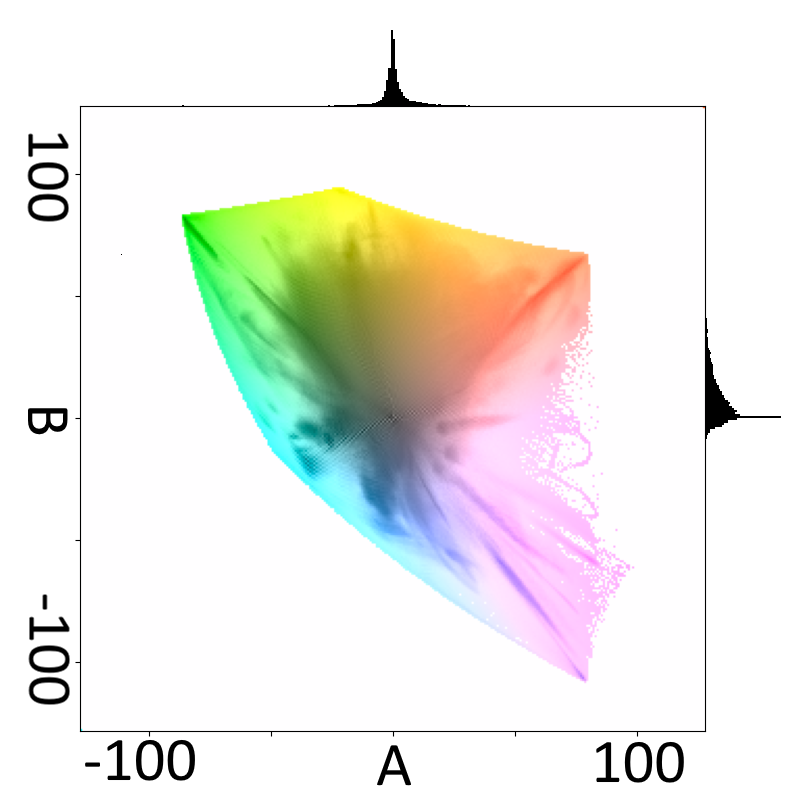
\includegraphics[width=\textwidth]{../code/dataAnalysis/plots/lab/DataCombined_lab.png}
            \caption{All Data}
        \else
            \includegraphics[width=\textwidth]{../code/dataAnalysis/plots/lab/labPlot_\i}
            \caption{source \i}
        \fi

        \label{fig:lab_sub\i}
      \end{subfigure}
      % Use the modulo operation to determine if a line break should be added
      \pgfmathparse{int(mod(\i+2,4))}
      \ifnum\pgfmathresult=0
          \newline
      \else
          \hfill
      \fi
    }
    \begin{subfigure}[t]{0.23\textwidth}
        \centering
        % No image to include, so this is left empty
        \caption*{} % Empty caption
    \end{subfigure}
    \caption*{}
    \addtocounter{figure}{-1}
\end{figure}

\begin{figure}[H]
    \centering
    \foreach \i in {19,...,33}{
      \begin{subfigure}[t]{0.23\textwidth}
        \centering       
        \ifnum \i=-1
            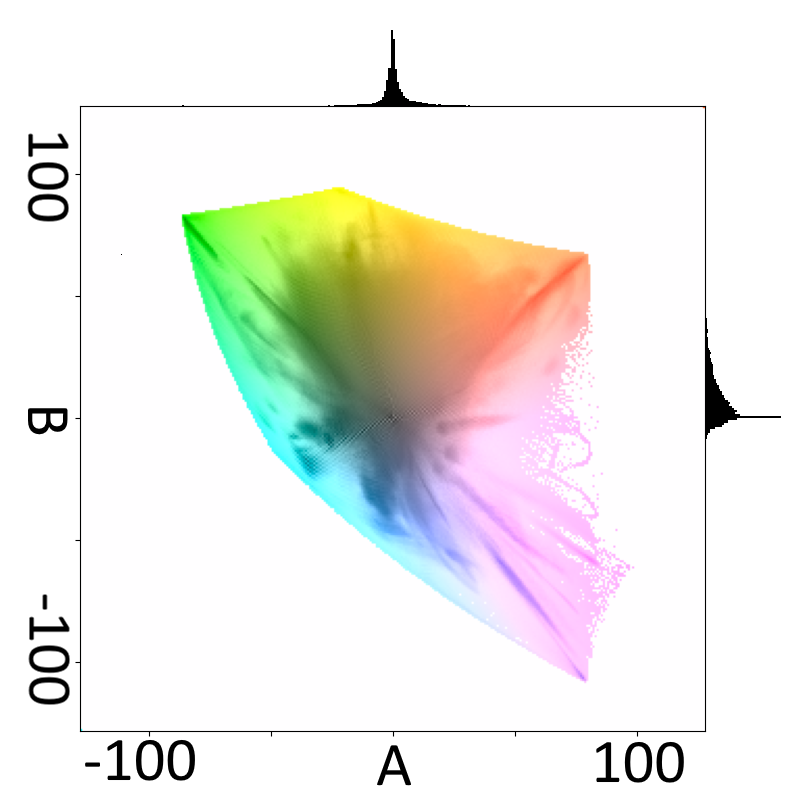
\includegraphics[width=\textwidth]{../code/dataAnalysis/plots/lab/DataCombined_lab.png}
            \caption{All Data}
        \else
            \includegraphics[width=\textwidth]{../code/dataAnalysis/plots/lab/labPlot_\i}
            \caption{source \i}
        \fi

        \label{fig:lab_sub\i}
      \end{subfigure}
      % Use the modulo operation to determine if a line break should be added
      \pgfmathparse{int(mod(\i+2,4))}
      \ifnum\pgfmathresult=0
          \newline
      \else
          \hfill
      \fi
    }
    \begin{subfigure}[t]{0.23\textwidth}
        \centering
        % No image to include, so this is left empty
        \caption*{} % Empty caption
    \end{subfigure}
    \caption{Visualization of datasets plotted in the LAB color space}
    \label{fig:lab_all2}

\end{figure}


\newpage

\subsection{Dataset Plots in the RGB Color Space}

\begin{figure}[H]
    \centering
    \foreach \i in {-1,...,18}{
      \begin{subfigure}[t]{0.23\textwidth}
        \centering

        \ifnum \i=-1
            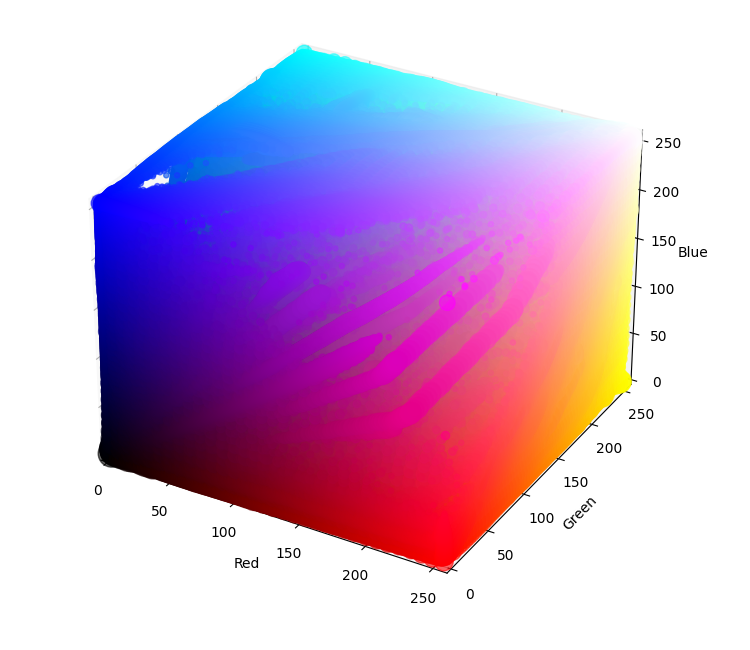
\includegraphics[width=\textwidth]{../code/dataAnalysis/plots/rgb/DataCombined_rgb.png}
        \caption{All Data}
        \else
            \includegraphics[width=\textwidth]{../code/dataAnalysis/plots/rgb/rgbPlot_\i}
            \caption{source \i}
        \fi
        \label{fig:rgb_sub\i}
      \end{subfigure}
      % Use the modulo operation to determine if a line break should be added
      \pgfmathparse{int(mod(\i+2,4))}
      \ifnum\pgfmathresult=0
          \newline
      \else
          \hfill
      \fi
    }
    \begin{subfigure}[t]{0.23\textwidth}
        \centering
        % No image to include, so this is left empty
        \caption*{} % Empty caption
    \end{subfigure}
    \caption*{}
    \addtocounter{figure}{-1}

\end{figure}

\begin{figure}[H]
    \centering
    \foreach \i in {19,...,33}{
      \begin{subfigure}[t]{0.23\textwidth}
        \centering

        \ifnum \i=-1
            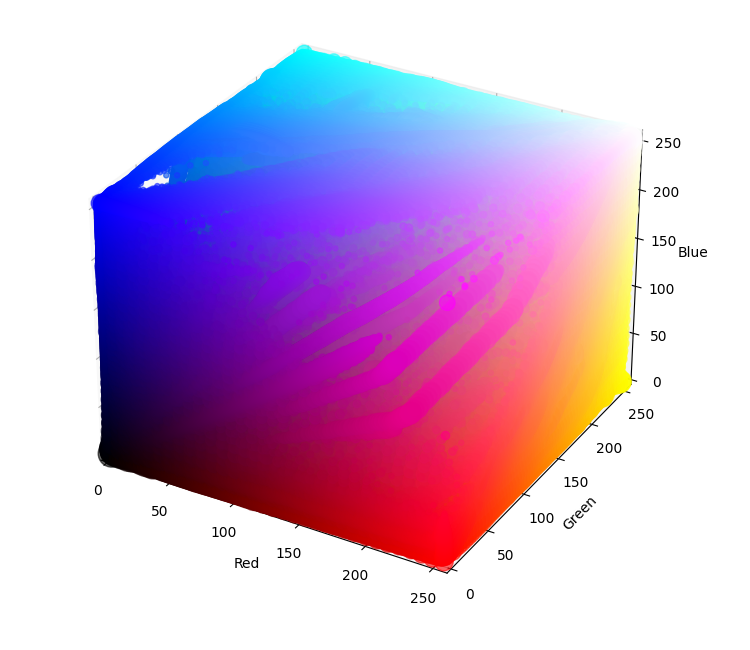
\includegraphics[width=\textwidth]{../code/dataAnalysis/plots/rgb/DataCombined_rgb.png}
        \caption{All Data}
        \else
            \includegraphics[width=\textwidth]{../code/dataAnalysis/plots/rgb/rgbPlot_\i}
            \caption{source \i}
        \fi
        \label{fig:rgb_sub\i}
      \end{subfigure}
      % Use the modulo operation to determine if a line break should be added
      \pgfmathparse{int(mod(\i+2,4))}
      \ifnum\pgfmathresult=0
          \newline
      \else
          \hfill
      \fi
    }
    \begin{subfigure}[t]{0.23\textwidth}
        \centering
        % No image to include, so this is left empty
        \caption*{} % Empty caption
    \end{subfigure}
    \caption{Visualization of datasets plotted in the RGB color space}
    \label{fig:rgb_all}

\end{figure}

\newpage
\begin{landscape}
\subsection{Trained Models with hyperparameters}
\label{sec:trained_models_hyperparameters}


    \begin{table}[H]
    \centering
    \caption{Model Configuration Overview}
    \scriptsize
    \begin{tabular}{|c|c|c|c|c|c|c|c|c|c|c|c|}
    \toprule
    MODEL & VER. & BATCH\_SIZE & BLOCK\_SIZE & N\_EMBD & N\_HEAD & N\_LAYER & DROPOUT & GPUS & DATASET & FINAL VAL\_LOSS & DURATION \\
    \midrule
    \multirow{2}{*}{\rotatebox{90}{CIT}} % Rotates CIT label by 90 degrees
    & 1.0 & 32 & 512 & 768 & 12 & 12 & 0.1 & 4 & ImageNet & 0.004 & 24h \\
    & 1.1 & 64 & 1024 & 1024 & 16 & 16 & 0.1 & 8 & CIFAR-10 & 0.004 & 12h \\
    \midrule
    \multirow{2}{*}{\rotatebox{90}{SIT}} % Rotates SIT label by 90 degrees
    & 1.0 & 32 & 512 & 768 & 12 & 12 & 0.1 & 4 & ImageNet & 0.004 & 24h \\
    & 1.1 & 64 & 1024 & 1024 & 16 & 16 & 0.1 & 8 & CIFAR-10 & 0.004 & 12h \\
    \bottomrule
    \end{tabular}
    \end{table}
\end{landscape}

\newpage

\subsection{Local workstation setup}

\begin{table}[H]
    \centering
    \begin{tabularx}{0.90\textwidth}{|X|X|}
    \hline
    \textbf{Component} & \textbf{Specification} \\ \hline
    Operating System & Microsoft Windows 11 Pro \\ \hline
    CPU & AMD Ryzen 9 7900X 12 cores, 4.7 GHz \\ \hline
    GPU & NVIDIA RTX 3090 \\ \hline
    RAM & 64 GB (DDR5-6000) \\ \hline
    SSD & 2TB Samsung 990 PRO M.2 PCIe 4.0 \\ \hline
    \end{tabularx}
    \caption{Local Workstation Setup}
    \label{table:workstation_setup}
\end{table}
    
\begin{table}[H]
    \centering
    \begin{tabularx}{0.90\textwidth}{|X|X|}
    \hline
    \textbf{Component} & \textbf{Specification} \\ \hline
    CPU & 2x Intel Xeon "Ice Lake" Platinum 8360Y (36 cores per socket, 2.4 GHz) \\ \hline
    GPU & 4x Nvidia A100 (80GB HBM2, SXM) \\ \hline
    RAM & 1 TB RAM (DDR4-3200) \\ \hline
    SSD & 7.68 TB NVMe local SSD \\ \hline
    \end{tabularx}
    \caption{Single compute node}
    \label{table:server_setup}
\end{table}

\newpage

\subsection{Transformer layer implementation}
\label{sec:transformer_layer_Python}

\begin{lstlisting}[language=Python]
class Head(nn.Module):
""" one head of self-attention """

    def __init__(self, head_size):
        super().__init__()
        self.key = nn.Linear(N_EMBD, head_size, bias=False)
        self.query = nn.Linear(N_EMBD, head_size, bias=False)
        self.value = nn.Linear(N_EMBD, head_size, bias=False)
        self.register_buffer('tril', torch.tril(torch.ones(BLOCK_SIZE, BLOCK_SIZE)))

        self.dropout = nn.Dropout(DROPOUT)

    def forward(self, x):
        # input of size (batch, time-step, channels)
        # output of size (batch, time-step, head size)
        B,T,C = x.shape
        k = self.key(x)   # (B,T,hs)
        q = self.query(x) # (B,T,hs)
        # compute attention scores ("affinities")
        wei = q @ k.transpose(-2,-1) * k.shape[-1]**-0.5 # (B, T, hs) @ (B, hs, T) -> (B, T, T)
        wei = wei.masked_fill(self.tril[:T, :T] == 0, float('-inf')) # (B, T, T)
        wei = F.softmax(wei, dim=-1) # (B, T, T)
        wei = self.dropout(wei)
        # perform the weighted aggregation of the values
        v = self.value(x) # (B,T,hs)
        out = wei @ v # (B, T, T) @ (B, T, hs) -> (B, T, hs)
        return out

class MultiHeadAttention(nn.Module):
""" multiple heads of self-attention in parallel """

    def __init__(self, num_heads, head_size):
        super().__init__()
        self.heads = nn.ModuleList([Head(head_size) for _ in range(num_heads)])
        self.proj = nn.Linear(head_size * num_heads, N_EMBD)
        self.dropout = nn.Dropout(DROPOUT)

    def forward(self, x):
        out = torch.cat([h(x) for h in self.heads], dim=-1)
        out = self.dropout(self.proj(out))
        return out

class FeedFoward(nn.Module):
""" a simple linear layer followed by a non-linearity """

    def __init__(self, n_embd):
        super().__init__()
        self.net = nn.Sequential(
            nn.Linear(n_embd, 4 * n_embd),
            nn.ReLU(),
            nn.Linear(4 * n_embd, n_embd),
            nn.Dropout(DROPOUT),
        )

    def forward(self, x):
        return self.net(x)

class Block(nn.Module):
""" Transformer block: communication followed by computation """

    def __init__(self, n_embd, n_head):
        # n_embd: embedding dimension, n_head: the number of heads we'd like
        super().__init__()
        head_size = n_embd // n_head
        self.sa = MultiHeadAttention(n_head, head_size)
        self.ffwd = FeedFoward(n_embd)
        self.ln1 = nn.LayerNorm(n_embd)
        self.ln2 = nn.LayerNorm(n_embd)

    def forward(self, x):
        x = x + self.sa(self.ln1(x))
        x = x + self.ffwd(self.ln2(x))
        return x
\end{lstlisting}

This code snippet shows the implementation of the transformer layer in the Column Image Transformer and the Spiral Image Transformer. The code above is heavily inspired by the implementation of the script by A.
Karpathy named NanoGPT \autocite{nanoGPTkarpathy2023} \autocite{nanogpt-lecturekarpathy2023}